\documentclass{article}
\usepackage{wrapfig}
\usepackage{float}
\usepackage{enumitem}
\usepackage{multirow}
\usepackage{longtable}
\usepackage{graphicx}
\usepackage{array}
\usepackage{amsmath}\usepackage{hyperref}
\graphicspath{ {report figures/} }
\usepackage{titlesec}
\usepackage[margin=1.5in]{geometry}
\geometry{a4paper, top=30mm, bottom=30mm}
\setlength{\skip\footins}{1cm}
\date{}
\author{He Ma u5893274}
\setlength{\parindent}{0pt}
\begin{document}
\title{\vspace{-1cm}System Engineering Assignment 3}
\maketitle
\section{Executive Summary}
To make a preliminary design for the power storage subsystem of 2030Yea project, 6 design criteria are selected to evaluate the performance of 3 potential design solutions. Each of the design criteria is the quantification of 1 to 2 system requirements (provided in appendix 2) which are derived from customer's needs. The technical performance measured (TPM) of each design criteria are set according to the requirements if they are numerically stated. Otherwise, the TPMs are set according to the average value of products on the market (TPMs are documented in appendix). Then the performance of each design option on each TPM are estimated by benchmarking or statistical modeling. Their performance scores are weighted by the importance of related requirements and improvement ratio with respect to benchmark and summed up to an overall score for each design options. Finally, for some design criteria where the performance of systems can vary randomly, the variance are added to or subtracted from the performance value to calculate a range of score for the design options. T-test are used to determine whether the variance of performance can  affect the decision making based on the mean overall scores of design options.\\
\\
Building a regional large scale power reserve seems to be the best solution based on the trade-off analysis mentioned above. But the decision cannot be made confidently due to a low T-test score. A potential solution is provided at the end of trade-off analysis section.
\section{Design Criteria}
\subsection{Energy Storage Capacity}
The most critical factor of a energy storage system is its capacity. It is also explicitly stated in R1.3 that the storage subsystem of 2030Yea's renewable energy system should be 7MWh. Regional electricity storage in design option A like Hornsdale Power Reserve has a fixed capacity (Hornsdale Power Reserve, 2018) far exceeding the value from the requirement while the community battery and household battery in other 2 design options are very flexible depending on the number of houses and communities. Such difference in capacity can be useful to discriminate design option A from other options.\\
\\
The direction of improvement (DoI) is no doubt positive, because larger capacity means more energy produced when there is sunlight can be stored and used when there is no sunlight. At minimum the storage should be able to deal with day and night cycle which means the minimum capacity is the energy consumption in 1 night for the whole town. By multiplying 16kWh which is the Australian average household daily consumption of electricity (SolarQuotes, 2024) with 1789 which is the population of Yea (city population, 2021) and divided by 2.5 which is the average population per household  (Agarwal, Bishop and Day, 2023), we can get the minimum capacity is 11.43MWh. The benefit of larger capacity diminish when the capacity goes to infinity. This is because a longer period of lacking sunlight is less likely to happen and the battery need just enough capacity to cover most of the time in a year. As R1.2 requires the system to fail no more than 1 time per year, the failing probability is \(\dfrac{1}{365}=0.3\%\). Assuming the weather being sunny is 50\%, the probability of 9 consecutive days without sunlight is \(0.5^9=0.20\%\) which is smaller than the required failing probability. The target capacity should be the energy consumption of 9 consecutive days which is also \(9\times 11.43MWh=102.87MWh\) (the daily consumption is calculated before for the minimum capacity). Any capacity larger than this value is not necessary for the requirements. Larger capacity won't reduce the performance of the system so there is no maximum capacity for this criterion.
\subsection{Voltage on Loads}
The voltage supplied to every load in the network is expected to meet AS 60038 standard issued by Standards Australia in 2000 where the nominal voltage is 230 volts with a +10\%, -6\% range (Commission Electrotechnique Internationale, 2008). Studies have shown that the voltage on household electrical appliances can vary greatly even if the designated output voltage from power source is 230 volts (Tripathy, 2008). This fact is mainly cause by sudden rise or drop of the total electricity load in the network. The topology of power supply distribution can greatly affect how load variation can be dealt with. Therefore the distinction of the 3 design options with very different battery distribution can be revealed by marking against this design criterion.\\
\\
The target voltage is set to 230, the minimum voltage is \(230v\times(1-6\%)=216.2v\) and maximum voltage is \(230v\times(1+10\%)=253v\), as they are required in AS 60038 standard (Commission Electrotechnique Internationale, 2008).
\subsection{Electromagnetic Emission Power}
Electromagnetic emission power is the commonly used measure to assess the electromagnetic compatibility of an electrical equipment. Only equipment meeting the IEC 61000-6-3 Generic standards - Emission standard for equipment in residential environments can be installed into the residential area in Australia (International Electrotechnical Commission, 2020). This standard restrict the power of electromagnetic wave emitted in a frequency range between 0-2kHz. The electromagnetic wave will be measured at distance of 3 meter from the power source. Because less emission is always better for safety considerations, the DoI is negative and there will be no minimum emission power. However the system should aim at 43.5dBuV/m which is the power emission limit for class B devices in the standard. At maximum the emitted electromagnetic wave from power source should be no greater than the class A power emission limit which is 49.5dBuV/m (International Electrotechnical Commission, 2020), otherwise the device is not safe to be installed in residential area.
\subsection{Power Efficiency}
Power efficiency is a measure of how much energy produced by solar panels can actually be used in electrical appliances. Because solar power produced per year is not going to be affected by power storage system, the power usage efficiency is going to be the dominant factor that affect the overall power output mentioned in R1.1. There are always power loss in the charging/discharging and transmission process. Concentrated large scale power reserve can balance the supply and consumption of power leading to less charging/discharging. However the long distance transmission from power reserve can cause higher loss of energy. This measure can reveal the overall power output performance of different designs by dividing the power consumption measured at microgrid controller by the power production measured at solar inverter.\\
\\Ideally, the power efficiency would be 100\%, so the DoI is positive and there is no maximum efficiency. The benchmark for worst case is the transmission efficiency of power plants which is at around 97\% (Chaplin, 2009). Since every bit of power efficiency is equally important for economy and environment, the target of power efficiency should also be 100\% so that any improvement of power efficiency get credited.
\subsection{Frequency Variation}
The power storage subsystem should comply with the Australian Frequency Operating Standard (Australian Energy Market Commission, 2017) as it is stated in R1.6. In addition, correct frequency output is essential for the connection to national grid which is mentioned in R2. The power frequency is mainly regulated by the control system of the power grid. Because the 3 design options adopt different methods to connect the microgrid controller with batteries. Their stability in terms of power frequency will be different. According to the standard mentioned above the maximum variation is 0.5Hz. The minimum variation is set to 0, representing exactly 50 Hz. Since a stable frequency is desired, the DoI is negative.
\subsection{Cost}
Whether the new energy system can save money for the residents of Yea is crucial. The cost here refers to the summation of installation cost and the maintenance cost in the next 25 years which is the life expectancy mentioned in R1.7. Lower cost is always desirable so the DoI is negative. Requirements R8.2 pointed out that the new system should benefit the local economy, so the maximum cost should be at least cheaper than the estimated electricity cost in the next 25 years without the new power system. This value can be estimated using benchmarking. The population growth in Australia can be modeled as a function of time: \(P(year)\) (Mcdonald and Siew-Ean Khoo, 2003) and the average electricity bill in Australia is around 1300 dollar per year. The electricity cost for all residents at Yea for the next 25 years is the summation of population each year times average bill: \(\Sigma_{year=2023}^{2048} 1300\times P(year)=97.8\) million AU\$. To meet the affordable requirement in R8.3, the target cost should be around 10\% construction cost of properties which is the average cost of solar power electrical system for properties across Australia (Boxwell, 2010). This value is calculated to be 35.78 million AU\$ using the average house construction cost (Yardney, 2020), total population in Yea (city population, 2021) and average population per household (city population, 2021).
\section{Requirements Matrix Allocations}
\begin{figure}[H]
\label{al}
\center
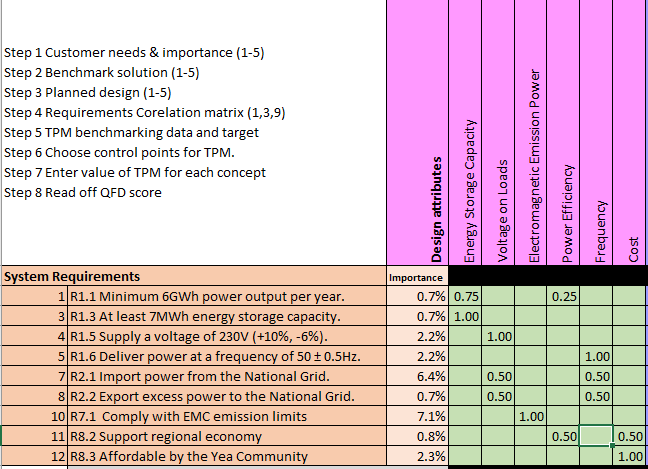
\includegraphics[scale=0.8]{allocation}
\caption{Requirements Matrix}
\end{figure}
As shown in the diagram above, some requirements relevant to the trade-off analysis of power storage subsystem are allocated to design criteria. The green area in the diagram shows the normalized correlation between each requirement and design criterion. The correlations are normalized so that each requirements has a total correlation of 1. This is because when a requirement correlates to multiple design criteria, its weight in the overall score can be scaled up or down depending how many criteria are correlated to the requirement. To avoid the bias of choosing design criteria, each requirement should have the same weight when calculating the score of a design. For the values in the matrix, 0.75 means major correlation, 0.25 means minor correlation, 0.5 means partial correlation and 1 means absolute correlation.\\
\\
The power output is directly related to the capacity of batteries, but with the same amount of power stored, a higher power efficiency can also increase the output by the amount of increased efficiency. Therefore the power efficiency is allocated with a minor correlation with power output requirement. For operating voltage and frequency, besides correlating to their explicitly corresponding requirements, ie R1.5 and R1.6, they are also essential for connecting to the national power grid. The national power grid operate strictly according the to the AS 60038 voltage standard and Australian Frequency Operating Standard. The power storage will not be allowed to connected to national grid without either correct voltage or frequency. So they have equal correlation to R2.1 and R2.2. The affordability is determined by the cost of the system while profitability is a synergy of cost and energy surplus which can be sold to benefit local economy. Suppose the cost of hardware and installation are invariant, then the cost to produce each unit of energy is fixed. The lost of energy inside the system now is the only factor can reduce profit. Hence R8.2 is equally correlated to cost and power efficiency.\\
\\
Because the trade-off between storage method mainly affect the capability and cost of the system, most of the requirement chosen are from R1 and R8. The 3 different design options also imply different transmission and regulation methods, therefore the requirement of connection to national grid is also included. R7.1 is included because the safety for batteries located inside community is an issue only for some design options and decisions should based on this trade-off as well.
\section{Trade-off Analysis}
Option A install a concentrated battery storage in regional area. Such type of power reserve will cost a lot to build but also provide huge amount of capacity. The Hornsdale Power Reserve can be considered as a benchmark where the capacity is 193.5 MW h while the cost is 172 million AU\$ (Hornsdale Power Reserve, 2018). Putting those numbers into the TPM developed in section 2 gives a score of 1 for capacity and 0 for cost. On the other hand community battery storage and household battery storage are flexible in terms of capacity, so their capacity can be set as the target vale. The average cost for household battery is 1150 AU\$ per kWh(Jeff Sykes 2024). Multiplying this number with the target capacity, we can get the cost for household batteries which is 118 million AU\$. For community batteries, the cost per kWh capacity should be similar to large concentrated power reserve. So it can be calculated by dividing the cost of Hornsdale Power Reserve by its capacity and multiply with the target capacity which result in 91.5 million AU\$.\\
\\
Along the transmission path through community, concentrated power supply may leads to an decreased voltage and power near the end of the transmission path (Tripathy, 2008). So the voltage for option A and B is set to 223V, in the middle between the target and minimum. For distributed batteries in household, the voltage can be stabled with the help of microgrid controller. So the voltage is set to 230 for option C.\\
\\
For distributed power supply, it is really hard to synchronize the frequency of each power source but the concentrated power supply are usually equipped with phase and frequency stabilizer to compensate the distortion caused by load (Tripathy, 2008). Therefore, the frequency variation for option A is set to 0.1Hz and for option C is set to 0.5Hz. Option B is a semi-distributed design so the frequency variation is set to 0.3Hz.\\
\\
Because the power of electromagnetic wave  dissipate in cubic speed as distance increases, large regional power reserve have almost no effect on residential area. The electromagnetic power for option A is set to 0. Household batteries are usually classified as type B electrical appliance (International Electrotechnical Commission, 2020). So the radiation power is set to 43.5 dBuV/m. The community batteries are relatively close to residential area comparing to regional power reserve, and its radiation is concentrated. So the radiation power is set to 49.5dBuV/m.\\
\\
The power efficiency for regional power reserve can be reduced by the bilateral transmission of the power. By multiplying the power transmission efficiency per kilometer (Pansini, 2020) with the radius of Yea town, the one way power efficiency can be calculated as 99\%. So the 2 way power efficiency is \(99^2\%=98\%\). The power efficiency of lithium-ion batteries is negligible, so the distributed household batteries almost have a 100\% power efficiency. The community batteries has a relatively shorter transmission distance so the power efficiency is set to 99\%.\\
\\
Due to unstable power load in the network, the voltage and frequency can be randomly varying in the range that is specified in their corresponding standards. Therefore, a stochastic decision test is applied by calculating the upper and lower limit of each design options. The upper limit of score is calculated with the values closest to the target and the lower limit is calculated with values farthest from the target. The result is shown in figure below, where the error bars indicates the possible score range due to random variables and the mid point of each bar represents the overall score of each design options. 
\begin{figure}[H]
\center
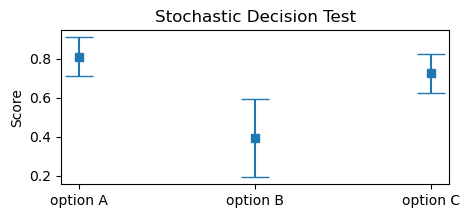
\includegraphics[scale=1]{err}
\end{figure}
Based on the variance and mean value of each design option, T-test can be conducted on each pair of options. The probability of option A and B have the same score is 0.05 which means there is a significant difference between option A and B. However the T-test yields a possibility of 0.28 that option A and C have the same score, so their score are indistinguishable.\\
\\
In conclusion, building a community based power storage can be ruled out because this design option have a significantly lower score. However, the house of quality analysis gives very similar score for regional power reserve and distributed household batteries. The T-test between these 2 options indicates that there is a 28\% possibility that regional power reserve is not the optimal solution despite that it has the highest score. By looking back at the requirement importance we can find that the scores are dominantly affected by the criteria that are related to electromagnetic radiation power and national grid connection. The differences between option A and C in terms of cost and capacity are not acknowledged sufficiently in the house of quality. To make a confident choice between option A and C, either the importance of requirements needs to be negotiated with clients or the benchmark needs to be adjusted so that the relative weight of capacity and cost related requirements can be increased.
\section*{Appendix 1: TPM}
\begin{figure}[H]
\center
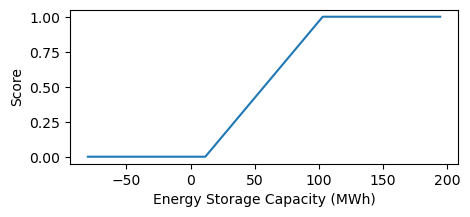
\includegraphics[scale=0.7]{tpm1}
\end{figure}
\begin{figure}[H]
\center
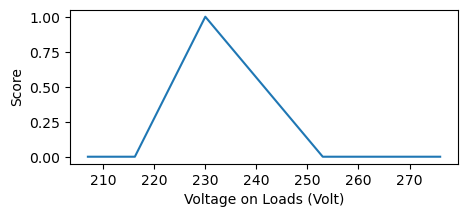
\includegraphics[scale=0.7]{tpm2}
\end{figure}
\begin{figure}[H]
\center
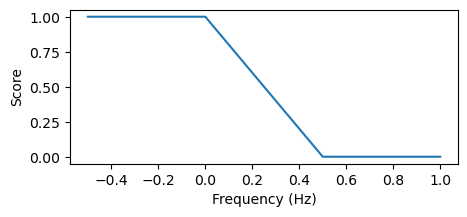
\includegraphics[scale=0.7]{tpm3}
\end{figure}
\begin{figure}[H]
\center
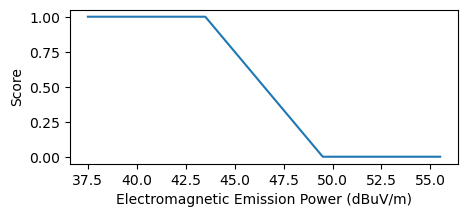
\includegraphics[scale=0.7]{tpm4}
\end{figure}
\begin{figure}[H]
\center
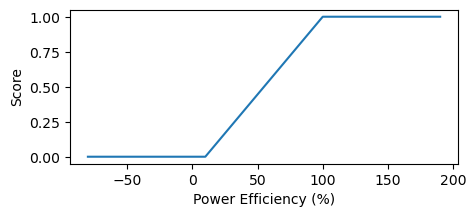
\includegraphics[scale=0.7]{tpm5}
\end{figure}
\begin{figure}[H]
\center
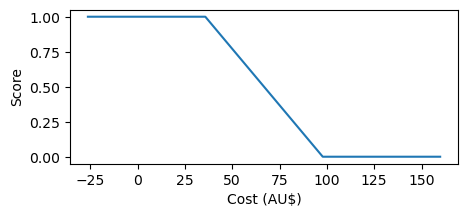
\includegraphics[scale=0.7]{tpm6}
\end{figure}
\section*{Appendix 2: List of System Requirements}
\textbf{R1} Capability\\
\textbf{R1.1} The system shall provide a minimum power output of 6GWh per year.\\
\textbf{R1.2} The system shall fail at most once per year.\\
\textbf{R1.3} The system shall have an energy storage capacity of 7MWh. \\
\textbf{R1.4} The system output shall grow at a rate of 2\% per year from the year 2023.\\
\textbf{R1.5} The system shall supply a voltage of 230V (+10\%, -6\%) to the customer\\
\textbf{R1.6} The system shall deliver power to the customer at a frequency of 50 ± 0.5Hz.\\
\textbf{R1.7} The system shall be planned for operation for at least 25 years from the date of installation \\
\textbf{R2} National Grid\\
\textbf{R2.1} The system shall import power from the National Grid as required. \\
\textbf{R2.2} The system shall export excess power to the National Grid. \\
\textbf{R3} Utility\\
\textbf{R3.1} The system shall support smart grid operation\\
\textbf{R3.2} The system shall support “Demand Response” \\
\textbf{R3.3} The system shall support EV Smart charging \\
\textbf{R3.4} The system shall enable the user to generate and consume their own local energy \\
\textbf{R4} Maintainability\\
\textbf{R4.1} The system shall be maintainable by local power provider technicians \\
\textbf{R4.2} The system shall be supportable with readily available materials\\
\textbf{R5} Energy Source\\
\textbf{R5.1} The system shall generate electricity from renewable energy sources\\
\textbf{R6} Infrastructure and Safety\\
\textbf{R6.1} The system shall distribute electricity via the currently installed distribution network\\
\textbf{R6.2} New infrastructure required by the system shall be integrated into the existing distribution network. \\
\textbf{R7} Safety\\
\textbf{R7.1} The system shall comply with EMC emission limits for MV and HV power systems \\
\textbf{R7.2} All new components of the system shall meet Australian safety standards \\
\textbf{R7.3} The system shall have adequate fault protection \\
\textbf{R8} Economics and Environment\\
\textbf{R8.1} The system shall not impact negatively on the health of the local environment\\
\textbf{R8.2} The systems installation and operation shall support the regional economy. \\
\textbf{R8.3} The system must be affordable by the Yea Community \\
\textbf{R8.4} The system shall support social equity through energy sharing \\
\textbf{R8.5} The system shall employ local businesses for its installation\\ 
\textbf{R8.6} The system shall employ local businesses for its maintenance\\ 
\section*{Bibliography}
Hornsdale Power Reserve (2018). \textit{Hornsdale Power Reserve.} [online] Hornsdalepowerreserve.com.au. Available at: https://hornsdalepowerreserve.com.au/.\\
\\
2030Yea (2021).\textit{2030Yea Annual Report}. Available at: https://2030yea.com.au/wp-content/uploads/2022/05/2030Yea-Annual-Report-2021.pdf.\\
\\
SolarQuotes (2024). \textit{How Many Batteries Do You need}. SolarQuotes | Get 3 Solar Quotes From Your Best Local Installers. [online] Available at: https://www.solarquotes.com.au/.\\
\\
city population (2021). \textit{City Population - Population Statistics in Maps and Charts for Cities, Agglomerations and Administrative Divisions of all Countries of the World.} [online] Available at: https://www.citypopulation.de/.\\
\\
Commission Electrotechnique Internationale (2008). Electrical installation guide : according to IEC international standards. Rueil-Malmaison (Bp 50604, 92506 Cedex): Schneider Electric, Merlin Gerin.\\
\\
Tripathy, S.C. (2008). Power electronics. New Delhi: Narosa.\\
\\
International Electrotechnical Commission (2020). \textit{Electromagnetic compatibility (EMC) - Part 6-3: Generic standards - Emission standard for residential, commercial and light-industrial environments}. (2007).\\
\\
Chaplin, R.A. (2009). \textit{Thermal Power Plants}. Encyclopedia of Life Support Systems.\\
\\
Australian Energy Market Commission (2017). \textit{The Frequency operating standard}. Australian Energy Market Commission.\\
\\
Mcdonald, P.F. and Siew-Ean Khoo (2003). \textit{The transformation of Australia’s population : 1970-2030}. Sydney: Unsw Press.\\
\\
Boxwell, M. (2010). \textit{Solar electricity handbook : a simple, practical guide to solar energy : designing and installing photovoltaic solar electric systems}. Ryton On Dunsmore, Warwickshire, U.K.: Greenstream Pub.\\
\\
Agarwal, N., Bishop, J. and Day, I. (2023). \textit{A New Measure of Average Household Size}. RESERVE BANK OF AUSTRALIA.\\
\\
Yardney, B. (2020). \textit{How Much Does It Cost to Build a House in Australia?} [online] Property Update. Available at: https://propertyupdate.com.au/how-much-on-average-does-it-cost-to-build-a-house/.\\
\\
Jeff Sykes (2024). \textit{Solar Batteries: Are They Worth It?} [online] Available at: \\https://www.solarchoice.net.au/solar-batteries/is-home-battery-storage-worth-it/.\\
\\
Pansini, A.J. (2020). \textit{Power Transmission \& Distribution, Second Edition}. CRC Press.
\end{document}